\section{Methods}
\subsection{The algorithm}
The algorithm scheme is described in Fig \ref{fig:1.png}.
\begin{figure}[H]
	\centering
	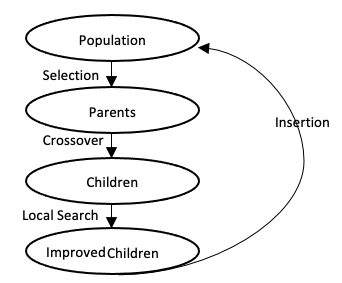
\includegraphics[width=0.4\textwidth]{1.png}
	\caption{Algorithm scheme. The population is initialized randomly.  In each
		iteration, first using tournament to select some best individuals according to fitness.
		Then crossover are performed on two individuals among the bests. Each
		generated child is improved individually using local search, and then new individuals are inserted to the population to replace the old
		individuals under some conditions. Iterate the process until a solution is
		found.						}
	\label{fig:1.png}
\end{figure}

\subsubsection{Representation}
A candidate solution is a string of bits whose length equals to the number of
variables of the considered problem instance. Every variable is associated to
one bit. This is the most obvious way to represent a solution candidate. It
also makes mutation and crossover operations computationally efficient. The
most successful evolutionary algorithms for SAT also uses representation
\parencite{gottlieb_marchiori_rossi_2002}. Hence the bit string representation is a reasonable
starting point.

\subsubsection{Fitness function}
The fitness value is equivalent to the number of satisfied clauses of the
individual.
\begin{equation*}
	\mathit{fitness}(x) = \sum_{i=1}^m c_i(x)
\end{equation*}
where $c_i(x)$ is the truth value of the $i$th
clause, and $m$ is the number of clauses.

\subsubsection{Selection operation}
GNTSAT uses a modified version of tournament selection. First, a certain
number of individuals are randomly select to participate in the tournament.
The participating individuals are ranked according to fitness. The most fit
individuals will be selected and stored in a best individuals pool. The two
parents will be selected randomly from this pool.

\subsubsection{Crossover operators}
The main goal of the crossover operator in GNTSAT is to create potentially
promising new individuals. Using the selected parents, there are many ways for
them to crossover, and we consider 5 types: CC (Corrective Clause) Crossover,
F\&F (Fleurent and Ferland) Crossover, Uniform Crossover, One-point Crossover
and Two-point Crossover. We will introduce them respectively below.

\begin{itemize}
	\item
	      CC (Corrective Clause) Crossover: For each clause c that is unsatisfiable for
	      both parent\_x and parent\_y solutions and for each variables that appears in
	      clause c, find the bit position using the literally absolute value
	      $i$ of the variable that produces the maximum improvement on
	      two parents guided by the improvement evaluation function. The function equals
	      to the number of false clauses which become true by flipping the
	      $ith$ bit in one of the solutions minus the number of
	      satisfied clauses which become false. Assign the flipped value applied to one
	      of the parents to the child in the bit position found, and all the bits with
	      no value of child take the value in corresponding position of parent\_x or
	      parent\_y with the equal probability.
	\item
	      F\&F (Fleurent and Ferland) Crossover: For each clause c that is satisfiable
	      for one parent and unsatisfiable for the other parent and for each variables
	      that appears in clause c, the bits positions in the child, corresponding to
	      the literally absolute value $i$ of the variable in parents,
	      are assigned values according to the parent satisfying the identified clause.
	      All the bits with no value of the child take the value in corresponding
	      position of parent\_x or parent\_y with the equal probability.
	\item
	      Uniform Crossover: With equal probability, each bits of the child is chosen
	      from either parent. In that case, one new offspring is generated.
	\item
	      One-point Crossover: Randomly select one pivot point (ranging between 0 to
	      length of the bits string) and exchange the substring from that bit point till
	      the end of the string between the two individuals. In that case, two new
	      offspring individual are generated.
	\item
	      Two-point Crossover: Randomly pick two pivot points and the bits in between
	      the two points are swapped between the parent individuals. In that case, two
	      new offspring individual are generated.
\end{itemize}

\subsubsection{Local search}
We implement the idea of mutation in genetic algorithm using WalkSAT local
search method. It is a stochastic local search algorithm. It attempts to
determine the best move by randomly choosing a clause among those that are
currently unsatisfied and selecting a variable to flip within it under some
conditions. The search stops when one solution is found.

\subsection{Implementation}
GNTSAT is implemented in C++. GNTSAT takes a DIMACS CNF file as input and
output the resulting bit string if found. User could adjust parameters such as
population size, tournament size, and crossover operator.

\subsection{Performance measures}
After all these processes to generate a solution, we compare our solver using
different crossovers and with other existing solvers. Several runs are
required for each benchmark instance under consideration and some measuring
methods need to be taken for statistically meaningful and also relatively fair
results. We take 10 runs and consider three measuring methods: SR (Success
rate), AT (Average Time) and AFS (Average Flips to Solution). We will
introduce them respectively below.

\begin{itemize}
	\item
	      SR (Success rate): SR represents the percentage of runs where a solution has
	      been found within a time limit. Since some runs where the time to get a
	      solution is too long or the solver is stuck in the local optimal solution, we
	      use SR to measure the quality of the solver. And the maximum time we set for a
	      successful run is 120 seconds.
	\item
	      AT (Average Time): AT represents the average seconds taken in successful runs.
	\item
	      AFS (Average Flips to Solution): Relating the computational costs to the
	      number of the basic moves in the search space for a solution has become the
	      standard measure used for studying the cost of SAT algorithms
	      \parencite{Singer2000}. AFS represents the average number of bit flips needed
	      to find a solution in successful runs, which was raised by
	      \citeauthor{Voss} and used to compare EAs generating new solution
	      candidates by single bit flips \parencite{Voss}.
\end{itemize}
